\chapter{ Data engineering workflow }

The aim of the chapter 2 is to lay the theoretical groundwork for constructing data pipelines. The typical workflow data engineer's undergone starts with data ingestion. The data engineer is responsible for collecting data from various sources such as databases, APIs, streaming platforms, or file systems. They set up data pipelines to extract data from these sources. Once the raw data is ingested, it is time to processes and transform it into a usable format. This involves cleaning the data, handling missing values, applying business logic or aggregations, and conforming the data to a defined schema. The goal is to make the data consistent, accurate and ready for analysis. Then, the processed data needs to be stored in a centralized repository for easy access. The data engineer designs and maintains the data storage infrastructure, which could include databases (relational or NoSQL), data warehouses, or data lakes. They optimize the storage for performance, scalability, and cost-efficiency. Data often needs to be combined from multiple sources to provide a unified view. The data engineer builds ETL (Extract, Transform, Load) or ELT (Extract, Load, Transform) pipelines to integrate data from different systems, applying necessary transformations and mappings to ensure data consistency. Ensuring the security, privacy, and integrity of the data is a critical responsibility. It is necessary to implement access controls, data encryption, and compliance measures. They also establish data governance policies and procedures to maintain data quality and lineage. Then data engineer creates mechanisms to make the data accessible to various stakeholders, such as data scientists, analysts, or business users. This could involve setting up APIs, query interfaces, or data visualization tools. They optimize data retrieval performance and ensure data is served in a format suitable for the intended use case. Lastly, they are continuously monitoring the data pipelines, storage, and serving layers to ensure smooth operation. They set up alerts, logging, and error handling to quickly identify and resolve issues. Regular maintenance tasks include updating data schemas, optimizing performance, and managing data growth\footnote[17]{\fullcite{konak2023hare}}\footnote[18]{\fullcite{kumariAnalysingMethodsWorkflow2023}}.

\section{Data quality dimensions}

Before diving into data processing frameworks, it should be clarified on the basis of what data quality is assessed. This subchapter focuses only on 5 data quality dimensions that are the most related to the thesis. However, in the cited paper, there are teens of dimension. Also, it could have been a lot to say about data validation, profiling, cleansing, enrichment, transformations, and frameworks, but this is beyond this master thesis\footnotemark[19].

Data quality dimensions encompass a range of attributes that define the quality and usability of data within a data pipeline. These dimensions serve as a framework, for evaluating and gauging the quality of data, including accuracy, completeness, consistency, timeliness, and uniqueness\footnotemark[19].

Accuracy pertains to how data reflects real-world entities or events it aims to represent. It gauges the proximity of data values to their true or expected values. Inaccurate data can lead to incorrect analyses, flawed decision-making, and unreliable insights. For example, in a customer database, ensuring that the recorded addresses and contact information are accurate and up to date\footnotemark[19].

Completeness assesses the extent to which all required data is present and available for analysis. It ensures that there are no missing values, fields, or records in the dataset. If the data is incomplete, it can hinder the effectiveness of data analysis and lead to biased or inaccurate results. For example, in a sales transaction dataset, ensuring that all necessary fields, such as customer ID, product ID, quantity, and price, are populated for each transaction\footnotemark[19].

Consistency pertains to how data's cohesively maintained across various sources, systems or time frames. It ensures that data is represented in a standardized format and follows defined business rules and constraints. Inconsistent data can lead to confusion, errors, and difficulties in data integration and analysis. For instance, one might standardize date formats across all data sources to a format (such as using ISO8601 "YYYY-MM-DD") to prevent misunderstandings and facilitate data integration\footnotemark[19].

Timeliness measures how fresh and accessible data is when required for analysis or decision-making. It ensures that data is current and reflects the most recent state of the entities or events it represents. Outdated or stale data can lead to incorrect insights and suboptimal decisions. As an example, may be a real-time fraud detection system, could ensure that transaction data is processed and analyzed in near-real-time to identify and prevent fraudulent activities promptly\footnotemark[19].

Lastly, the uniqueness refers to the absence of duplicate records or entities within a dataset. It guarantees that each record or entity is singularly represented, preventing redundancy and inconsistency. Duplicate data can skew analysis results, consume storage space, and lead to incorrect aggregations. In a customer relationship management (CRM) system, one may implement deduplication techniques to identify and merge duplicate customer records based on unique identifiers or matching criteria\footnote[19]{\fullcite{andrewblackDimensionsDataQuality2020}}.

\section{Data ingestion}

Data ingestion refers to the process of collecting and importing data from various sources into a data storage system or processing pipeline. It involves capturing data from diverse origins, such as databases, files, streaming platforms, and IoT devices, and making it available for further processing and analysis\footnote[16]{\fullcite{Kona2023LeveragingSA}}.

Data ingestion often deals with \textbf{large volumes} of data generated at high velocities, such as real-time streaming data or high-throughput transactional systems. Ingesting and processing such data requires scalable data ingestion frameworks. Data can come in \textbf{various formats}, such as structured (such as CSV, JSON), semi-structured (like XML, log files), and unstructured (e.g., text, images, videos). Data ingestion processes need to handle and parse these diverse formats to extract meaningful information. Another case is that data pipelines need to be \textbf{resilient to failures and ensure data reliability}. They should handle network disruptions, system failures, and data inconsistencies gracefully, without losing data or compromising data integrity\footnotemark[16].

The simplest is \textbf{batch ingestion}. It involves collecting and importing data in batches at regular intervals.  Distributed processing frameworks like Apache Spark enable batch ingestion, allowing for the processing of large datasets in parallel across a cluster of machines. Another approach is \textbf{real-time streaming}, it deals with capturing and processing data as it arrives, enabling near-real-time analysis and decision-making. Streaming frameworks like Apache Kafka, Apache Flink, and Akka Streams are tools for building these pipelines. The last approach to mention is \textbf{Change Data Capture (CDC)}. CDC is a technique that captures and replicates changes made to a source database in real-time. It enables the ingestion of incremental updates and ensures data consistency between the source and target systems. Frameworks, such as Debezium and Apache Kafka Connect, facilitate CDC-based data ingestion\footnotemark[16].

\section{Data processing}

The initial stage of data processing involves the acquisition of raw data from a multitude of sources, both internal and external to the organization. These sources can range from transactional databases and operational systems to web logs, social media feeds, and IoT sensor networks. The data may be structured, semi-structured, or unstructured, necessitating a robust and scalable ingestion framework capable of handling diverse data formats and volumes. Data engineers must design and implement efficient pipelines to extract, transfer, and load this data into a centralized repository or data lake for further processing\footnote[10]{\fullcite{Kona2023LeveragingSA}}.

Raw data is often plagued with issues such as inconsistencies, duplicates, missing values, and errors, which can significantly impact the quality and reliability of downstream analysis. The data cleaning phase aims to identify and rectify these anomalies through a series of techniques, including data deduplication, handling missing values through imputation or deletion, data type conversion, and outlier detection and treatment. This process ensures that the data adheres to predefined quality standards and is suitable for subsequent transformation and analysis\footnotemark[10].

Once the data has been cleaned and validated, it undergoes a transformation process to convert it into a format optimized for analysis and storage. This stage may involve various operations, such as data normalization, aggregation, joining data from multiple sources, feature engineering, and data enrichment. The transformed data is typically structured in a denormalized or dimensional format, facilitating efficient querying and analysis. Data engineers must carefully design and implement these transformation pipelines, considering factors such as performance, scalability, and maintainability\footnotemark[10].

With the processed and transformed data, data analysts and scientists can perform a range of analytical techniques to derive insights and support data-driven decision-making. This may involve statistical analysis, machine learning, data mining, and data visualization. Data engineers collaborate closely with these stakeholders to ensure that the processed data meets their requirements and can be seamlessly integrated into their analytical workflows\footnotemark[10].

The final stage of data processing involves storing the processed and transformed data in a format optimized for querying and future use. This often involves loading the data into data warehouses, data marts, or NoSQL databases, depending on the specific requirements of the organization. Data engineers design and implement the storage schemas, indexing strategies, and partitioning techniques to ensure optimal performance, scalability, and cost-efficiency for analytical workloads\footnotemark[10].

\section{Data storage systems}

\subsubsection{The importance of data storage}

In the modern business world, data is considered the lifeblood that drives organizations forward. Today, companies understand that data plays a crucial role in their business intelligence systems, enabling them to make informed decisions and maintain a competitive advantage in their respective industries\footnotemark[20]. Companies generate, collect, and process massive volumes of data, frequently falling under the category of big data. Managing and analyzing this data effectively is essential for deriving valuable insights and supporting data-driven decision-making\footnotemark[20]. With the unprecedented growth in data volume and variety, traditional data storage approaches face limitations. Handling and examining the immense quantity and diversity of big data can be a challenging and complex undertaking. However, when an organization effectively harnesses and leverages its extensive data repository, it can uncover valuable insights that inform and guide its business strategies\footnotemark[20]. To address these challenges, organizations require efficient and scalable data storage solutions. Data warehouses and data lakes have emerged as popular data management systems for storing and managing big data\footnotemark[20].

Data warehouses (DW) and data lakes (DL) serve as centralized repositories for storing and managing an organization's data\footnotemark[20]. While DW and DL share some similarities, they differ in their characteristics and application. They also have distinct characteristics that make them suitable for different data storage and analysis requirements\footnotemark[20].  DW stores data in a structured and organized manner, often using predefined schemas. They are designed for structured data and are optimized for fast querying and analysis. In contrast, DL stores data in its raw format, allowing for the storage of structured, semi-structured, and unstructured data\footnotemark[20]. Another aspect is efficiency.  A relational model has scalability problems, causing rapid performance decreases when data volume increases. One of the solutions was a new data model. NoSQL databases, such as key-value stores, column-oriented databases, document stores, and graph databases, were designed as alternatives to traditional relational databases. They offer scalability, flexibility, and performance advantages for handling big data\footnote[21]{\fullcite{Nayak2013TypeON}}.

\textbf{Data storage systems} play a main role in data pipelines by serving as the foundation for storing, managing and accessing data at various stages of the pipeline. The \textbf{scalability factor} is crucial in highlighting the significance of these systems. As data volumes continue to grow exponentially, data storage systems must be able to scale horizontally to accommodate the increasing storage requirements. Distributed storage solutions like Apache Hadoop HDFS and Amazon S3 are designed to scale by adding nodes to the cluster, allowing efficient handling of massive datasets. These systems offer fault tolerance and data replication mechanisms to ensure data availability and durability, even during the hardware failures. Additionally, scalable data storage systems support the construction of data pipelines that can handle the ever-growing demands of big data applications, making it easier to store and analyze terabytes or petabytes of information. The ability to dynamically \textbf{scale storage capacity} without downtime or performance issues is critical for maintaining performance and reliability in managing increasing data volumes and complexities, within data pipelines\footnote[20]{\fullcite{Nambiar2022AnOO}}.

\subsection{The role and challenges associated with storing}

During the \textbf{data ingestion phase}, data storage systems serve as the hub for receiving data from various sources, like databases, files, APIs and streaming services. They must manage the high volume and velocity of data to ensure reliable and efficient storage. Handling scalability is a challenge during this phase, as storage systems must expand to accommodate increasing data volumes without sacrificing performance or data integrity. Distributed storage systems such as Apache Hadoop HDFS and Amazon S3 are designed to scale horizontally by adding more nodes to the cluster, allowing for the storage and processing of extensive datasets\footnotemark[20].

In the data processing stage, data storage systems act as both the source and destination for data transformations and computations. They need to provide fast access to stored data to support data processing tools in retrieving and manipulating information effectively. Performance plays a role at this stage, since storage systems need to meet high throughput and low latency demands for handling data processing workloads efficiently. Distributed storage systems combined with parallel processing frameworks like Apache Spark enable the processing of large datasets by distributing both data and computations across multiple nodes, in the cluster\footnotemark[20].

Data \textbf{consistency} is another significant challenge when storing and managing large-scale data. With multiple processes and users accessing and modifying the data concurrently, ensuring data consistency and integrity becomes crucial. Data storage systems need to provide mechanisms for maintaining data consistency, such as \textbf{ACID} (Atomicity, Consistency, Isolation, Durability) properties in traditional databases or eventual \textbf{consistency models} in distributed systems. Techniques like data partitioning, replication, and versioning help in maintaining data consistency and enabling fault tolerance in the face of failures or network partitions.

In the \textbf{data serving phase}, data storage systems act as the backbone for delivering processed and aggregated data to downstream applications and users. They need to support fast and efficient querying and retrieval of data, often in real-time or near-real-time scenarios. Scalability and performance are critical in this phase, as data storage systems must be able to handle a high volume of concurrent queries and deliver results with low latency. \textbf{Distributed databases}, such as Apache Cassandra and Apache HBase, are designed to provide scalable and high-performance data serving capabilities, enabling fast access to large datasets.

\subsection{Types of data storage systems}

\subsubsection{Data warehouses}

Data warehouses serve as centralized repositories for storing and managing large volumes of structured data from various sources. They are designed to support complex queries, data analysis, and reporting, enabling organizations to gain valuable insights from their data\footnote[20]{\fullcite{Nambiar2022AnOO}}.

\begin{enumerate}
    \item They typically follow a \textbf{schema-on-write approach}, where the data schema is defined upfront, and data is transformed and validated before being loaded into the warehouse. This ensures data consistency and integrity, as the data conforms to a predefined structure\footnotemark[20].
    \item Data warehouses are optimized for \textbf{Online Analytical Processing (OLAP)} workloads, which involve complex queries, aggregations, and multidimensional analysis. They provide features like indexing, partitioning, and materialized views to facilitate efficient querying and analysis of large datasets\footnotemark[20].
    \item They are designed to \textbf{handle complex queries} that involve joining multiple tables, aggregating data, and performing calculations. They provide SQL-based query interfaces and support advanced query optimization techniques to ensure fast query execution. Examples of data warehouses: Amazon Redshift, Google BigQuery, Snowflake\footnotemark[20].
\end{enumerate}

\subsubsection{Data lakes}

Data lakes are another component of data storage systems. They provide a centralized repository for storing vast amounts of raw, unstructured, and semi-structured data from various sources, enabling organizations to leverage the power of big data analytics\footnote[20]{\fullcite{Nambiar2022AnOO}}.

\begin{enumerate}
    \item Data lakes differ from data warehouses in their approach, to handling schemas. While data warehouses use a schema-on-write method, data lakes employ a \textbf{schema-on-read} paradigm. In terms, data in a data lake is stored in its form without a predefined schema upon ingestion. The schema is applied when the data is accessed and processed, offering flexibility to adapt to evolving data needs\footnotemark[20].
    \item Data lakes have the capability to store data in various formats, including structured data (like CSV and JSON), semi structured (such as XML and log files) and unstructured (e.g., images and videos) formats. This versatility allows organizations to collect and retain information from sources like social media platforms, IoT devices and clickstream datasets\footnotemark[20].
    \item Cost-effective storage of volumes of data is a feature of data lakes. They make use of distributed storage systems like Apache Hadoop HDFS or cloud services such as Amazon S3 and Azure Data Lake Storage for scalability, resilience and cost efficiency. These systems enable storing data, on hardware or cloud infrastructure, while ensuring reliability. Popular examples of data lakes include Apache Hadoop HDFS, Amazon S3 and Azure Data Lake Storage\footnotemark[20].
\end{enumerate}

\subsubsection{NoSQL databases}

NoSQL databases have gained significant popularity in recent years due to their ability to handle unstructured and semi-structured data efficiently. They provide a flexible and scalable alternative to traditional relational databases, making them well-suited for handling the diverse and rapidly growing data requirements of modern data pipelines\footnote[21]{\fullcite{Nayak2013TypeON}}.

\begin{enumerate}
    \item NoSQL databases offer a \textbf{schema-less} or \textbf{schema-flexible} approach, allowing for the storage of data without a predefined schema. This flexibility enables the easy accommodation of evolving data structures and facilitates the rapid development and iteration of data-driven applications\footnotemark[21].
    \item NoSQL databases are designed to scale horizontally, distributing data across multiple nodes in a cluster. They provide high-performance and low latency for read and write operations, making them suitable for handling large volumes of data and high-throughput workloads\footnotemark[21].
    \item NoSQL databases support various data models, including key-value, document, column-family, and graph. Each data model is optimized for specific use cases and provides different ways of organizing and querying data. Examples of NoSQL databases: Apache Cassandra, MongoDB, Apache HBase\footnotemark[21].
\end{enumerate}

\section{Data integration}

Data integration refers to the process of combining data from multiple sources into a unified view or format. It involves resolving inconsistencies, transforming data structures, and ensuring data quality and consistency across different systems.

In general, data sources are \textbf{heterogeneous}, meaning data often resides in various systems, such as databases, files, APIs, and streaming platforms, each with its own data format, schema, and access mechanisms. Integrating data from these diverse sources requires handling different data formats, protocols, and APIs. What's more, data from different sources may have inconsistencies, duplicates, missing values, or conflicting information. Data integration processes need to address these issues through data cleansing, deduplication, and data validation techniques. \textbf{Data schemas} may evolve over time, with changes in data structures, field names, or data types. Data integration pipelines need to be resilient to schema changes and capable of handling schema evolution gracefully, without breaking downstream processes.

ETL and ELT architectures are a common approach for data integration, where data is extracted from source systems, transformed into a consistent format, and loaded into a target system. ETL processes can be implemented using big data frameworks like Apache Spark. Another approach is accessing and retrieving data through \textbf{API}. Scala's libraries, such as Akka HTTP and Play Framework, provide tools for integrating with RESTful APIs, enabling seamless data integration from web services and cloud platforms. Lastly, data virtualization provides a unified view of data without physically moving or copying the data. It involves creating a virtual layer that abstracts the complexity of underlying data sources and presents a consistent interface for querying and accessing data. Scala's support for building scalable and performant data access layers makes it well-suited for implementing data virtualization solutions.

\subsection{Data pipeline architectures}

ETL (Extract, Transform, Load) and ELT (Extract, Load, Transform) are two fundamental data processing paradigms used in data engineering to extract data from various sources, transform it into a suitable format, and load it into target systems such as data warehouses or data lakes\footnote[16]{\fullcite{etleltDatacamp}}.

\begin{figure}[H].
\caption{ETL and ELT}
\centering
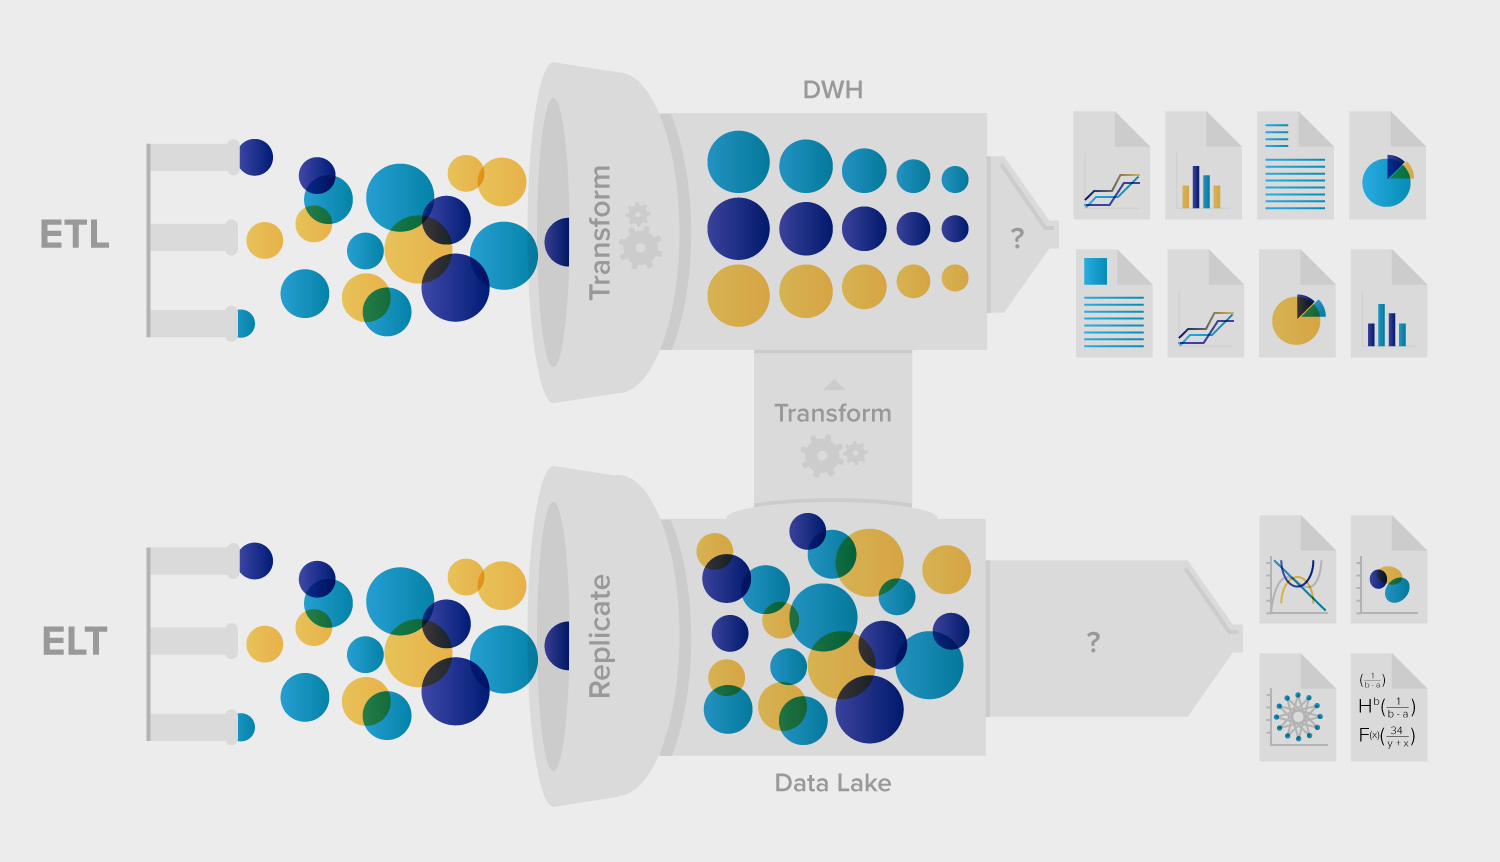
\includegraphics[width=1\linewidth]{images/image.png}
\small
\textit{Creator:} Datacamp. Retrieved June 15, 2024, from https://www.datacamp.com/blog/etl-vs-elt
\end{figure}

\subsection{ETL (Extract, Transform, Load)}
ETL is a process where data is first extracted from source systems, then transformed into a consistent format, and finally loaded into the target system\footnotemark[17].

\begin{itemize}
    \item In the extraction phase, data is collected from diverse sources such as databases, files, APIs, or streaming platforms. This step involves handling different data formats, ensuring data consistency, and dealing with data quality issues\footnotemark[17].
    \item The transformation phase is where the extracted data undergoes cleansing, validation, and restructuring to fit the schema of the target system. Common transformations include data type conversions, data enrichment, data aggregation, and applying business rules or logic\footnotemark[17].
    \item After the transformation, the data is loaded into the target system, typically a data warehouse or data lake. This phase considers factors such as data volume, data integrity, and data availability\footnotemark[17].

\end{itemize}

ETL is often preferred when the source data requires significant transformations or when the target system has limited processing capabilities. It allows for complex data transformations to be performed before loading the data, ensuring a consistent structure in the target system\footnotemark[17].

\subsection{ELT (Extract, Load, Transform)}
ELT is an alternative approach where the data is first extracted from the source systems and loaded directly into the target system, with the transformations occurring after the loading process\footnotemark[17].

\begin{itemize}
    \item The extraction and loading phases are similar to ETL, where data is collected from various sources and loaded into the target system. However, in ELT, the data is loaded in its raw format without any prior transformations\footnotemark[17].
    \item The transformation phase in ELT takes place within the target system itself, leveraging its processing power and capabilities. This allows for more flexible and scalable data transformations, as the target system can handle large volumes of data efficiently\footnotemark[17].
\end{itemize}

ELT is gaining popularity with the rise of big data and cloud computing platforms. It enables faster data loading and allows for more agile data processing, as transformations can be applied on-demand based on specific requirements. However, ELT also presents challenges such as ensuring data quality and handling schema evolution in the target system. It requires robust data governance and data validation mechanisms to maintain data integrity\footnotemark[17].

\subsection{Comparison of ETL and ELT}
When choosing between ETL and ELT, several factors come into play, including the complexity of data transformations, the processing capabilities of the destination system and the specific requirements of the data pipeline. \textbf{ETL} is an option, when the source data requires complex transformations or when the target system lacks processing power. It ensures that data is standardized before loading, maintaining quality and integrity. On the other hand, \textbf{ELT} is more suitable for handling large volumes of data and when the destination system has sufficient processing capabilities. It enables faster data loading and provides flexibility in applying transformations based on specific use cases\footnote[17]{\fullcite{etleltDatacamp}}.

\section{Data security and governance}
Data has become one of the most valuable assets for organizations today. As data volumes grow exponentially across disparate systems, effectively governing and managing data quality is critical for gaining accurate business insights and \textbf{maintaining regulatory compliance}. Poor quality data can obscure genuine insights and lead to flawed business decisions (\cite{Achanta2023DataGA})\footnotemark[23]. \textbf{Data governance} provides the overall strategy, policies, standards, and processes to ensure high-quality, secure, and compliant data assets across the organization. It aligns regulatory, operational, and strategic objectives with data management practices. Key activities include developing data policies, standards, and procedures; governing data models, metadata, and quality; providing clear data ownership and stewardship; and monitoring data usage and access for security and compliance (\cite{Achanta2023DataGA}).

\textbf{Data security} is a core component of governance. With growing cybersecurity threats and strict data protection regulations like \textbf{GDPR}, organizations must implement robust security controls within data platforms. This includes fine-grained access policies, data encryption, activity monitoring, and data loss prevention capabilities. Data classification and handling standards ensure sensitive data is adequately protected (\cite{Achanta2023DataGA})\footnotemark[23]. In data engineering pipelines, large volumes of data flow through various stages from ingestion to consumption. Data engineers have a pivotal role in embedding governance and quality validations within data infrastructure and processes. Robust data validation at ingestion, data cleansing and standardization within ETL workflows, data quality checks in analytics, and data lineage and cataloging are key focus areas (\cite{Achanta2023DataGA})\footnotemark[23].

Lack of data governance leads to data silos, inconsistent data definitions, poor metadata, and inadequate compliance. This hampers data sharing, erodes trust in data, and increases regulatory risks. Implementing a well-designed data governance framework, with representation from business, IT, and compliance teams, is essential. Processes and responsibilities for defining critical data elements, reference data, data quality rules, and resolving data issues must be established\footnote[24]{\fullcite{Xie2021SolutionIA}}. Emerging technologies offer new opportunities to scale governance. Machine learning can automate complex data matching, profiling quality, and detecting anomalies. Metadata management tools enable auto-classification, data lineage, and impact analysis. Data catalogs provide business glossaries and data dictionaries for users to discover and understand data assets. Cloud-based data governance services provide templates and workflows to jumpstart initiatives(\cite{Achanta2023DataGA})\footnote[23]{\fullcite{Achanta2023DataGA}}.

\section{Data serving}

Data pipelines are crucial for operationalizing machine learning by automating the flow of data from source to model training to inference. For real-time applications, the pipeline must seamlessly integrate stream processing with model serving, which is not always straightforward due to gaps in tooling. Serving ML models on streaming data is especially challenging when the models need to be continuously updated through online learning. MLOps practices like model versioning, monitoring, auditing, and zero-downtime updates are essential. Scalable architectures leveraging stream processing platforms like Kafka along with model serving frameworks enable dynamic learning in production. The performance of the model serving setup has a big impact on end-to-end latency and throughput. Comparative benchmarking is necessary to understand the subtle differences between various streaming and serving tools. Hardware acceleration through GPUs can provide a significant boost for some workloads. An emerging trend is the use of semantic technologies to simplify ML pipeline development and usage. Capturing domain knowledge and ML best practices in ontologies, exposed through intelligent modules and intuitive interfaces, allows non-ML experts to effectively leverage data science. This is valuable in industrial settings. In summary, robust data pipelines that can reliably process, update, and serve ML models on streaming data are essential for modern data-driven applications. While the ideal architecture is highly use-case dependent, adhering to MLOps best practices and using semantically enhanced tooling where possible helps navigate the implementation challenges. Careful benchmarking ensures the pipeline meets its performance objectives.\footnote[26]{\fullcite{Cdola2021FeatureEA}}

\section{Monitoring and maintenance}

Data pipelines form the backbone of machine learning systems by automating the flow of data from ingestion to model training and inference. A well-architected data pipeline ensures that ML models are provided with timely, high-quality data to learn from. Monitoring data pipelines is crucial to catch issues early and maintain the overall health of the system. This involves tracking metrics on data volume, schema changes, data distribution, and pipeline performance. Anomaly detection techniques can be applied to identify sudden changes and alert engineers. During pipeline development, substantial effort goes into feature engineering and transforming raw data into features for ML models. This could involve aggregating transaction records, extracting sentiment from text, calculating time-series statistics, etc. The quality of features has a big impact on model performance. With data coming from many sources in different formats, pipelines need to be adaptable. For unstructured data like video, specialized techniques may be needed, such as filtering video frames based on quality and content to create a representative training dataset. Cloud platforms have made it easier than ever to deploy data pipelines at scale. Managed services handle infrastructure provisioning and orchestration, so data engineers can focus on pipeline logic. Tools like Kubeflow help stitch together pipeline components. Data versioning is also an area of active development. Being able to track the version of data used to train a specific model is important for reproducibility and debugging. Pipeline metadata collection and data lineage tracking enable this. Finally, a major use case is using ML pipelines for predictive maintenance in industries like manufacturing, energy, and transportation. By analyzing sensor data and event logs, models can predict equipment breakdowns in advance, allowing repairs to be scheduled proactively. This improves reliability and reduces costs. In summary, monitoring, and maintenance are vital for the smooth operation of data pipelines, which in turn enables the success of data-driven initiatives across industries. A combination of good system design, vigilant monitoring, and proactive maintenance is needed to keep the data flowing \footnote[25]{\fullcite{roychowdhury2021videodata}}.